\chapter{Project Requirements}
This chapter describes the functional and non-functional requirements of the PawPal pet care mobile application. The requirements are gathered through use case analysis, stakeholder, and competitive analysis of existing pet care solutions.

\section{Use Case Analysis}
PawPal is an interactive end-user mobile application, making use case modeling the most appropriate requirement gathering technique. The following use cases represent the core functionalities across all eight modules of the system.

\subsection{System-Wide Use Case Diagram}

Figure \ref{fig:use_case_system_wide} illustrates the complete system-wide use case diagram for PawPal, showing all primary actors (Pet Owner, Veterinarian, Pet Caregiver, Marketplace Seller, and System Administrator) and their interactions with the system's core functionalities. The diagram also depicts the integration with external systems including Payment Gateway, AI/ML System, Email System, and GPS Service.

\begin{figure}[H]
    \centering
    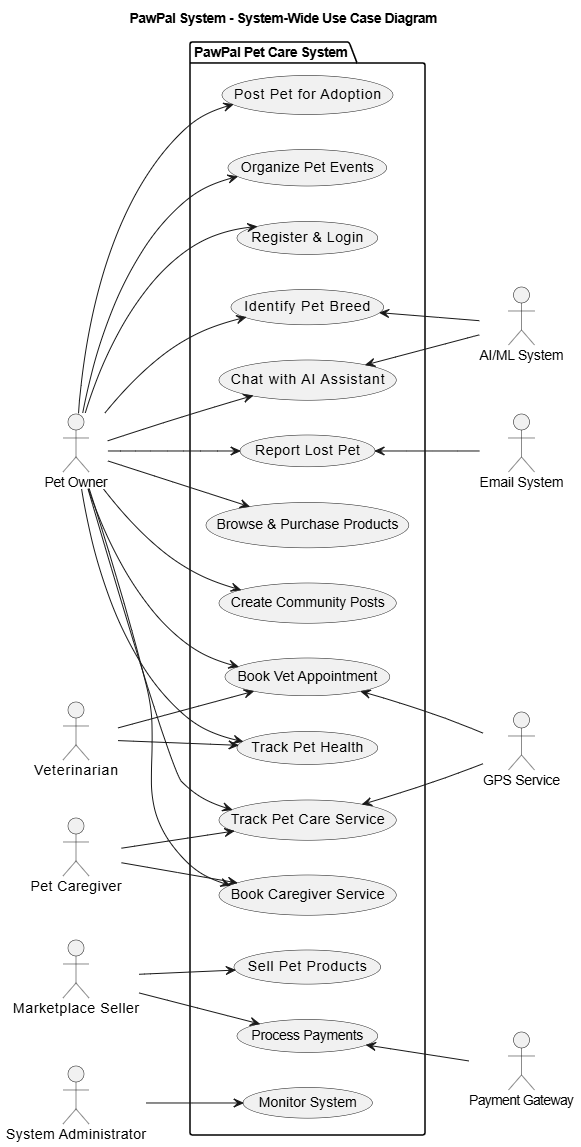
\includegraphics[width=\textwidth]{ThesisFigs/use_case.png}
    \caption{PawPal Use Case Diagram}
    \label{fig:use_case_system_wide}
\end{figure}

\subsection{High-Level Use Cases Overview}

The PawPal system supports twelve primary use cases that span across all eight modules, providing comprehensive pet care functionality:

\begin{enumerate}
    \item \textbf{User Registration and Authentication} - New users create accounts and existing users authenticate to access system features
    \item \textbf{Pet Breed Identification} - AI-powered breed recognition from uploaded pet photos with personalized care recommendations
    \item \textbf{AI Chatbot Consultation} - 24/7 virtual veterinary assistant providing instant health guidance and emergency support
    \item \textbf{Pet Profile Management} - Comprehensive digital pet profiles with health records, vaccination tracking, and journal maintenance
    \item \textbf{Marketplace Commerce} - End-to-end e-commerce for pet products including browsing
    \item \textbf{Veterinary Services} - Appointment booking, clinic discovery, and consultation management with healthcare providers
    \item \textbf{Caregiver Services} - Professional pet care service booking with real-time tracking and service completion verification
    \item \textbf{Community Participation} - Social networking features including posts, groups, events, and content sharing
    \item \textbf{Lost Pet Alert System} - Emergency alert broadcasting with community engagement and GPS-based notifications

    \item \textbf{Payment Processing} - Secure payment gateways using cryptocurrency transactions
    \item \textbf{System Administration} - Platform management including  dispute resolution, blocking users, handling payment errors 
\end{enumerate}

These high-level use cases encompass all stakeholder interactions including Pet Owners, Veterinarians, Caregivers, Marketplace Sellers, and System Administrators, ensuring comprehensive coverage of the PawPal ecosystem.

\subsection{Fully Dressed Use Cases}

The following detailed use cases follow the comprehensive use case template, providing complete specifications for each core system functionality.

\textbf{UC-0: User Registration and Authentication}

\textbf{Use Case ID:} UC-00

\textbf{Use Case Name:} User Account Registration and Login

\textbf{Scope:} PawPal Pet Care System

\textbf{Level:} User-goal level

\textbf{Primary Actor:} New User / Existing User

\textbf{Stakeholders and Interests:}
\begin{itemize}
    \item Users: Want simple, secure account creation and reliable authentication
    \item System Administrators: Require secure user management and fraud prevention
\end{itemize}

\textbf{Preconditions:} User has mobile device with internet connection and valid email address.

\textbf{Postconditions:} User account is created or authenticated with active session and dashboard access.

\textbf{Main Success Scenario:}
\begin{enumerate}
    \item User opens application and selects registration or login option
    \item User enters credentials (email, password) and accepts terms if registering
    \item System validates credentials and security requirements
    \item System sends email verification for new accounts
    \item User confirms email verification if registering
    \item System creates secure JWT session and grants dashboard access
\end{enumerate}

\textbf{Extensions (Alternate Flows):}
\begin{itemize}
    \item 2a. Invalid credentials or weak password: System displays error with requirements
    \item 3a. Login fails or account locked: System increments counter and requires password reset
    \item 4a. Email verification fails: System resends verification email
\end{itemize}

\textbf{Special Requirements:}
\begin{itemize}
    \item Security: bcrypt password hashing with cost factor 12, JWT tokens with 24-hour expiration
    \item Performance: Authentication completion within 5 seconds
\end{itemize}

\textbf{Technology and Data Variations:} JWT authentication, email-based password reset, future support for social login (Google/Apple) and multi-factor authentication.

\textbf{UC-1: Identify Pet Breed}

\textbf{Use Case ID:} UC-01

\textbf{Use Case Name:} AI-Powered Pet Breed Identification

\textbf{Scope:} PawPal Pet Care System

\textbf{Level:} User-goal level

\textbf{Primary Actor:} Pet Owner

\textbf{Stakeholders and Interests:}
\begin{itemize}
    \item Pet Owner: Wants accurate breed identification and personalized care recommendations
    \item Veterinarians: Benefit from accurate breed information for health guidance
\end{itemize}

\textbf{Preconditions:} User is logged in with camera permissions and pet image available.

\textbf{Postconditions:} Breed is identified, stored in database, and linked to pet profile with care recommendations.

\textbf{Main Success Scenario:}
\begin{enumerate}
    \item User captures or uploads pet photo (JPEG/PNG, max 10MB)
    \item System validates image quality and format
    \item System processes image through CNN model within 5 seconds
    \item System displays breed identification with confidence score (0-100\%)
    \item System provides breed characteristics and care recommendations
    \item User confirms and saves breed information to pet profile
\end{enumerate}

\textbf{Extensions (Alternate Flows):}
\begin{itemize}
    \item 2a. Invalid format or poor quality: System requests supported format or better image
    \item 4a. Confidence below 85\%: System provides top 3 alternative breed matches
    \item 6a. User disagrees: User can manually correct breed identification
\end{itemize}

\textbf{Special Requirements:}
\begin{itemize}
    \item Performance: Processing completion within 5 seconds
    \item Accuracy: CNN model maintains minimum 85\% accuracy on test datasets
\end{itemize}

\textbf{Technology and Data Variations:} CNN model (TensorFlow/PyTorch), JPEG/PNG with automatic compression, support for various camera resolutions.

\textbf{UC-2: Chat with AI Assistant}

\textbf{Use Case ID:} UC-02

\textbf{Use Case Name:} AI Chatbot Veterinary Consultation

\textbf{Scope:} PawPal Pet Care System

\textbf{Level:} User-goal level

\textbf{Primary Actor:} Pet Owner

\textbf{Stakeholders and Interests:}
\begin{itemize}
    \item Pet Owner: Wants immediate, accurate veterinary guidance for health concerns
    \item Veterinarians: Interested in quality referrals for complex cases
\end{itemize}

\textbf{Preconditions:} User is logged in with active internet connection and operational chatbot service.

\textbf{Postconditions:} User receives veterinary guidance with logged conversation and appropriate escalation if needed.

\textbf{Main Success Scenario:}
\begin{enumerate}
    \item User opens chatbot interface and submits pet care question
    \item System processes query through NLP and RAG pipeline
    \item System retrieves relevant veterinary knowledge from curated databases
    \item System generates contextual LLM response within 5 seconds
    \item System provides guidance with source citations and confidence score
    \item System logs conversation and allows follow-up questions
\end{enumerate}

\textbf{Extensions (Alternate Flows):}
\begin{itemize}
    \item 2a. Emergency keywords detected: System provides immediate emergency vet contacts
    \item 4a. LLM confidence below 70\%: System escalates to human veterinarian
    \item 4b. Response timeout: System apologizes and suggests retry
\end{itemize}

\textbf{Special Requirements:}
\begin{itemize}
    \item Performance: Response generation within 5 seconds, 24/7 availability with 99.5\% uptime
    \item Accuracy: Medical advice includes disclaimers and source citations
\end{itemize}

\textbf{Technology and Data Variations:} RAG pipeline with LLM (OpenAI GPT or similar), curated veterinary knowledge base, session history for contextual responses.

\textbf{UC-3: Create and Manage Pet Profile}

\textbf{Use Case ID:} UC-03

\textbf{Use Case Name:} Comprehensive Pet Profile Management

\textbf{Scope:} PawPal Pet Care System

\textbf{Level:} User-goal level

\textbf{Primary Actor:} Pet Owner

\textbf{Stakeholders and Interests:}
\begin{itemize}
    \item Pet Owner: Wants centralized digital record for comprehensive pet care management
    \item Veterinarians/Caregivers: Need accurate pet health history for consultations and services
\end{itemize}

\textbf{Preconditions:} User is logged in with pet information available.

\textbf{Postconditions:} Complete pet profile is created, stored securely, and accessible from dashboard.

\textbf{Main Success Scenario:}
\begin{enumerate}
    \item User selects "Add New Pet" from dashboard
    \item User enters mandatory details (name, species, breed, date of birth)
    \item User adds optional information (weight, microchip ID, insurance)
    \item User uploads up to 50 photos with automatic thumbnail generation
    \item System creates profile with unique ID and stores in database
    \item System displays profile summary and makes it accessible from dashboard
\end{enumerate}

\textbf{Extensions (Alternate Flows):}
\begin{itemize}
    \item 2a. Mandatory fields missing: System highlights required fields
    \item 4a. Photo upload fails or exceeds limit: System compresses or allows later upload
    \item 5a. Database save fails: System retries and notifies user
\end{itemize}

\textbf{Special Requirements:}
\begin{itemize}
    \item Storage: Support 50 photos per pet with automatic thumbnail generation
    \item Performance: Profile creation within 30 seconds, encrypted data at rest
\end{itemize}

\textbf{Technology and Data Variations:} JPEG/PNG with automatic compression, PDF export for vet appointments, cross-device synchronization.

\textbf{UC-4: Purchase Pet Products}

\textbf{Use Case ID:} UC-04

\textbf{Use Case Name:} Marketplace Product Purchase

\textbf{Scope:} PawPal Pet Care System

\textbf{Level:} User-goal level

\textbf{Primary Actor:} Pet Owner (Buyer)

\textbf{Stakeholders and Interests:}
\begin{itemize}
    \item Pet Owner: Wants secure, convenient product purchasing with reliable delivery
    \item Marketplace Seller: Needs efficient order processing and payment reception
\end{itemize}

\textbf{Preconditions:} User is logged in with active product listings and available payment method.

\textbf{Postconditions:} Order is placed, payment processed, seller notified, and delivery tracking initiated.

\textbf{Main Success Scenario:}
\begin{enumerate}
    \item User browses marketplace and applies filters (breed, price, ratings)
    \item User selects product, reviews details, and adds to cart
    \item User proceeds to checkout and selects payment method
    \item System calculates total with taxes, fees, and shipping
    \item User confirms payment and system processes through secure gateway
    \item System notifies seller and sends order confirmation with tracking to buyer
\end{enumerate}

\textbf{Extensions (Alternate Flows):}
\begin{itemize}
    \item 2a. Product out of stock: System suggests alternatives
    \item 5a. Payment fails or insufficient funds: System retries and notifies user
    \item 6a. Seller cancels: System processes automatic refund
\end{itemize}

\textbf{Special Requirements:}
\begin{itemize}
    \item Performance: Checkout completion within 60 seconds
    \item Reliability: 99.9\% payment processing uptime
\end{itemize}

\textbf{Technology and Data Variations:} Cryptocurrency (Bitcoin, Ethereum, USDT) and digital wallets, real-time order tracking via push notifications.

\textbf{UC-5: Book Veterinary Appointment}

\textbf{Use Case ID:} UC-05

\textbf{Use Case Name:} Veterinary Appointment Booking

\textbf{Scope:} PawPal Pet Care System

\textbf{Level:} User-goal level

\textbf{Primary Actor:} Pet Owner

\textbf{Stakeholders and Interests:}
\begin{itemize}
    \item Pet Owner: Wants convenient appointment scheduling with qualified veterinarians
    \item Veterinary Clinic: Needs efficient appointment management and calendar integration
\end{itemize}

\textbf{Preconditions:} User is logged in with pet profile created and clinics registered in system.

\textbf{Postconditions:} Appointment is scheduled with confirmations sent to both parties and calendar entries created.

\textbf{Main Success Scenario:}
\begin{enumerate}
    \item User searches for nearby clinics using GPS location
    \item System displays clinics on map with distance, ratings, and specializations
    \item User filters by specialization and views real-time availability
    \item User selects clinic, chooses appointment slot, and describes visit reason
    \item System sends booking request to clinic for confirmation
    \item System sends confirmations and integrates with pet health journal
    \item User receives appointment reminders 24 hours and 2 hours before time
\end{enumerate}

\textbf{Extensions (Alternate Flows):}
\begin{itemize}
    \item 2a. No nearby clinics: System expands search or suggests telemedicine
    \item 5a. Veterinarian declines or no slots: System suggests alternatives
    \item 7a. User reschedules or cancels: System allows changes with 4-hour notice
\end{itemize}

\textbf{Special Requirements:}
\begin{itemize}
    \item Availability: Real-time appointment updates with no double-booking
    \item Notifications: Multi-channel reminders (email, push) at 24h and 2h intervals
\end{itemize}

\textbf{Technology and Data Variations:} OpenStreetMap for clinic discovery, calendar sync with device and clinic systems, telemedicine for non-emergency cases.

\textbf{UC-6: Hire Pet Caregiver}

\textbf{Use Case ID:} UC-06

\textbf{Use Case Name:} Professional Pet Caregiver Service Booking

\textbf{Scope:} PawPal Pet Care System

\textbf{Level:} User-goal level

\textbf{Primary Actor:} Pet Owner

\textbf{Stakeholders and Interests:}
\begin{itemize}
    \item Pet Owner: Wants reliable, verified pet care services with real-time tracking
    \item Pet Caregiver: Needs efficient booking system with secure payment processing
\end{itemize}

\textbf{Preconditions:} User is logged in with pet profile, verified caregiver available, and payment method ready.

\textbf{Postconditions:} Service is booked, caregiver confirmed, payment processed, and tracking activated.

\textbf{Main Success Scenario:}
\begin{enumerate}
    \item User posts service request with dates, duration, and requirements
    \item System matches with verified caregivers in area
    \item User reviews caregiver profiles (ratings, certifications) and selects preferred
    \item Caregiver accepts request and user pays deposit
    \item System activates GPS tracking and communication channels
    \item Caregiver provides service with real-time updates
    \item Caregiver submits completion report, user reviews and releases payment
    \item Both parties submit ratings and feedback
\end{enumerate}

\textbf{Extensions (Alternate Flows):}
\begin{itemize}
    \item 2a. No caregivers available: System expands search area
    \item 4a. Caregiver declines or payment fails: System suggests alternatives
    \item 6a. Emergency during service: System activates emergency protocols
\end{itemize}

\textbf{Special Requirements:}
\begin{itemize}
    \item Security: Background verification with ID and reference checks
    \item Tracking: GPS updates every 2 minutes with route history
\end{itemize}

\textbf{Technology and Data Variations:} GPS tracking with route history, secure escrow payment system, in-app messaging with photo/video sharing.

\textbf{UC-7: Participate in Community}

\textbf{Use Case ID:} UC-07

\textbf{Use Case Name:} Community Hub Social Participation

\textbf{Scope:} PawPal Pet Care System

\textbf{Level:} User-goal level

\textbf{Primary Actor:} Community Member (Pet Owner)

\textbf{Stakeholders and Interests:}
\begin{itemize}
    \item Community Members: Want to share experiences and connect with other pet owners
    \item Content Moderators: Ensure safe, appropriate community environment
\end{itemize}

\textbf{Preconditions:} User is logged in with community guidelines accepted and content creation permissions.

\textbf{Postconditions:} Content is published, visible to appropriate audience, and engagement tracking activated.

\textbf{Main Success Scenario:}
\begin{enumerate}
    \item User creates new post selecting content type (text, image, video, poll)
    \item User adds content (up to 2000 characters, 10 images)
    \item User adds location tags, hashtags, and sets visibility (public/friends/groups)
    \item System performs automated moderation and policy compliance check
    \item System publishes post to community feeds
    \item Community members engage (like, comment, share) and user receives notifications
    \item System tracks engagement metrics for content algorithms
\end{enumerate}

\textbf{Extensions (Alternate Flows):}
\begin{itemize}
    \item 4a. Content flagged or policy violation: Post held for review with user feedback
    \item 6a. Group requires approval: Request sent to moderators
\end{itemize}

\textbf{Special Requirements:}
\begin{itemize}
    \item Moderation: Automated scanning with human escalation
    \item Performance: Real-time notifications within 10 seconds
\end{itemize}

\textbf{Technology and Data Variations:} Text, images, videos (60 seconds), polls, engagement analytics, cross-platform social sharing.

\textbf{UC-8: Process Payment}

\textbf{Use Case ID:} UC-08

\textbf{Use Case Name:} Secure Multi-Method Payment Processing

\textbf{Scope:} PawPal Pet Care System

\textbf{Level:} User-goal level

\textbf{Primary Actor:} Pet Owner (Payer)

\textbf{Stakeholders and Interests:}
\begin{itemize}
    \item Pet Owner: Wants secure, convenient payment processing with transaction records
    \item Service Provider/Seller: Needs reliable payment reception with fraud protection
\end{itemize}

\textbf{Preconditions:} User has initiated transaction with available payment method and validated amount.

\textbf{Postconditions:} Payment is processed, funds transferred, transaction recorded, and confirmations sent.

\textbf{Main Success Scenario:}
\begin{enumerate}
    \item System calculates total (cost, taxes, fees)
    \item User reviews summary and selects payment method (cryptocurrency, digital wallet)
    \item System generates wallet address/QR code (crypto) or processes via gateway (digital)
    \item User confirms and authorizes transaction
    \item System processes payment with fraud detection and validates completion
    \item System sends confirmation with transaction ID, credits provider account
    \item System updates status and generates audit trail
\end{enumerate}

\textbf{Extensions (Alternate Flows):}
\begin{itemize}
    \item 3a. Network congested or insufficient funds: System provides wait time or suggests alternatives
    \item 5a. Payment fails or fraud detected: System retries with backoff or holds for review
    \item 6a. Crediting fails: System queues retry and notifies recipient
\end{itemize}

\textbf{Special Requirements:}
\begin{itemize}
    \item Performance: Processing within 5 seconds with 99.9\% uptime
    \item Compliance: Transaction logging and audit trails
\end{itemize}

\textbf{Technology and Data Variations:} Cryptocurrency (Bitcoin, Ethereum, USDT), digital wallets with credit storage, multi-currency support, biometric authentication.

\textbf{UC-9: Create Lost Pet Alert}

\textbf{Use Case ID:} UC-09

\textbf{Use Case Name:} Emergency Lost Pet Alert System

\textbf{Scope:} PawPal Pet Care System

\textbf{Level:} User-goal level

\textbf{Primary Actor:} Pet Owner

\textbf{Stakeholders and Interests:}
\begin{itemize}
    \item Pet Owner: Needs immediate, wide-reaching alert to locate missing pet
    \item Community Members/Shelters: Want to help locate lost pets in area
\end{itemize}

\textbf{Preconditions:} User is logged in with pet profile created and GPS location available.

\textbf{Postconditions:} Alert is broadcasted to community and shelters with sighting reports enabled.

\textbf{Main Success Scenario:}
\begin{enumerate}
    \item User reports pet as missing and selects from profile list
    \item User provides last known location (GPS or manual) and uploads photos
    \item User sets urgency level and special medical needs
    \item System validates alert and broadcasts push notifications to community (5km radius)
    \item System sends email alerts to animal shelters (10km) and creates social posts
    \item Community receives alerts with photo and contact information
    \item System enables sighting reports with photo verification
    \item User receives real-time notifications of sightings
\end{enumerate}

\textbf{Extensions (Alternate Flows):}
\begin{itemize}
    \item 2a. GPS unavailable or no photos: User provides manual entry or uses profile photos
    \item 4a. No nearby community: System expands alert radius
    \item 8a. Pet found: User marks alert as resolved
\end{itemize}

\textbf{Special Requirements:}
\begin{itemize}
    \item Urgency: Alert broadcasting within 60 seconds
    \item Reach: GPS-based targeting with 5km community and 10km shelter radius
\end{itemize}

\textbf{Technology and Data Variations:} GPS coordinates with radius-based targeting, social media integration, AI-assisted photo verification for sightings.

\textbf{UC-10: Process Pet Adoption}

\textbf{Use Case ID:} UC-10

\textbf{Use Case Name:} Pet Adoption Process Management

\textbf{Scope:} PawPal Pet Care System

\textbf{Level:} User-goal level

\textbf{Primary Actor:} Prospective Pet Adopter

\textbf{Stakeholders and Interests:}
\begin{itemize}
    \item Prospective Adopter: Wants to find suitable pet and complete adoption process
    \item Animal Shelter: Needs efficient adoption workflow with proper screening
\end{itemize}

\textbf{Preconditions:} User is registered with shelters having listed adoptable pets and established criteria.

\textbf{Postconditions:} Adoption is completed with signed legal documents and pet profile transferred to new owner.

\textbf{Main Success Scenario:}
\begin{enumerate}
    \item User browses adoption listings with filters (species, breed, age, location)
    \item User views pet profiles (photos, health records, temperament)
    \item User submits application with personal information
    \item System performs screening and shelter reviews with reference checks
    \item Shelter schedules meet-and-greet session
    \item Shelter approves based on compatibility assessment
    \item User completes paperwork, pays fees, and receives pet care guide
    \item System transfers ownership and schedules 30-day follow-up
\end{enumerate}

\textbf{Extensions (Alternate Flows):}
\begin{itemize}
    \item 4a. Application incomplete or denied: System requests info or provides feedback
    \item 6a. Compatibility concerns: Shelter suggests alternative pets
    \item 7a. Payment fails: System holds adoption pending resolution
\end{itemize}

\textbf{Special Requirements:}
\begin{itemize}
    \item Verification: Background and reference checking with digital signatures
    \item Support: Post-adoption resources and 30-day follow-up
\end{itemize}

\textbf{Technology and Data Variations:} Automated screening with manual review, digital contracts and legal paperwork, adoption fee processing with receipts.

\section{Functional Requirements}
This section describes the functional requirements of PawPal organized by the eight core modules. Each requirement is expressed in natural language with specific, measurable, and testable criteria.

\subsection{Pet Identification Module}
The Pet Identification module is trained on Stanford Dogs and Oxford-IIIT Pets datasets to provide accurate breed detection capabilities.

\begin{enumerate}
    \item \textbf{FR-PI-1:} The system shall allow users to capture or upload pet images in JPEG, PNG, formats with maximum file size of 10MB.
    \item \textbf{FR-PI-2:} The system shall process uploaded images through a CNN model and return breed identification within 5 seconds.
    \item \textbf{FR-PI-3:} The system shall display breed identification results with a confidence score (0-100\%) and provide up to 3 alternative breed matches when confidence is below 85\%.
    \item \textbf{FR-PI-4:} The system shall provide detailed breed information including characteristics, temperament, care requirements, and common health issues.
    \item \textbf{FR-PI-5:} The system shall allow users to confirm or correct breed identification and save results to pet profiles.
    \item \textbf{FR-PI-6:} The system shall maintain a history of all breed identification attempts linked to user accounts.
\end{enumerate}

\subsection{Chatbot Module}
The Chatbot module implements Retrieval-Augmented Generation (RAG) combined with Large Language Models (LLM) to provide 24/7 intelligent pet care assistance.

\begin{enumerate}
    \item \textbf{FR-CB-1:} The system shall provide a conversational interface accepting text in English.
    \item \textbf{FR-CB-2:} The system shall process user queries through RAG pipeline to retrieve relevant veterinary knowledge from curated databases.
    \item \textbf{FR-CB-3:} The system shall generate contextual responses using LLM within 5 seconds of query submission.
    \item \textbf{FR-CB-4:} The system shall provide source citations and references for medical advice to ensure credibility.
    \item \textbf{FR-CB-5:} The system shall recognize emergency situations and provide immediate guidance with vet clinic recommendations.
    \item \textbf{FR-CB-6:} The system shall maintain conversation history for each user and allow resuming previous conversations.
    \item \textbf{FR-CB-7:} The system shall escalate complex medical queries to human veterinarians when confidence threshold drops below 70\%.
\end{enumerate}

\subsection{Pet Profiles \& Journals Module}
This module provides comprehensive digital record-keeping capabilities.

\begin{enumerate}
    \item \textbf{FR-PP-1:} The system shall allow users to create unlimited pet profiles with mandatory fields: name, species, breed, date of birth.
    \item \textbf{FR-PP-2:} The system shall support optional profile fields including weight, color, microchip ID, insurance details, and dietary restrictions.
    \item \textbf{FR-PP-3:} The system shall enable users to upload up to 50 photos per pet profile with thumbnail generation.
    \item \textbf{FR-PP-4:} The system shall maintain vaccination records with reminder notifications sent 7 days before due dates.
    \item \textbf{FR-PP-5:} The system shall track health milestones including vet visits, weight changes, and medical procedures with timeline visualization.
    \item \textbf{FR-PP-6:} The system shall provide digital journal functionality for daily activity logs, behavior notes, and mood tracking.
   
\end{enumerate}

\subsection{Pet Toy Marketplace Module}
The Marketplace module implements a full-featured e-commerce platform.

\begin{enumerate}
    \item \textbf{FR-MP-1:} The system shall allow verified sellers to list products with title, description, price, images (up to 10), and inventory quantity.
    \item \textbf{FR-MP-2:} The system shall categorize products into: Toys, Food, Accessories, Grooming, Healthcare, Apparel, and Training Equipment.
    \item \textbf{FR-MP-3:} The system shall provide advanced filtering by breed compatibility, price range, brand, ratings, and seller location.
    \item \textbf{FR-MP-4:} The system shall implement search functionality and  relevance-based ranking.
    \item \textbf{FR-MP-5:} The system shall maintain shopping cart with session persistence for 7 days.
    \item \textbf{FR-MP-6:} The system shall calculate total cost including product price, shipping fees, and applicable taxes.
    \item \textbf{FR-MP-7:} The system shall enable buyer reviews and ratings (1-5 stars) for completed orders.
\end{enumerate}

\subsection{Community Hub Module}
The Community Hub implements social networking features.

\begin{enumerate}
    \item \textbf{FR-CH-1:} The system shall allow users to create posts with text (up to 2000 characters), images (up to 10), and videos (up to 60 seconds).
    \item \textbf{FR-CH-2:} The system shall provide news feed with ranking based on recency, and user engagement.
    \item \textbf{FR-CH-3:} The system shall enable social interactions including likes, comments, and shares.
    \item \textbf{FR-CH-4:} The system shall implement hashtag functionality for content discovery and trending topics.
    \item \textbf{FR-CH-5:} The system shall provide event creation and management for pet meetups, adoption drives, and awareness campaigns.
    \item \textbf{FR-CH-6:} The system shall implement real-time push notifications for  comments, and event reminders.
    \item \textbf{FR-CH-7:} The system shall provide content moderation tools including report, block.
\end{enumerate}

\subsection{Veterinary Services Integration Module}
This module manages veterinary appointments and records.

\begin{enumerate}
    \item \textbf{FR-VS-1:} The system shall allow veterinary clinics to register with profile information including specializations, services, hours, and contact details.
    \item \textbf{FR-VS-2:} The system shall display vet clinics on a map with distance calculation from user's current location.
    \item \textbf{FR-VS-3:} The system shall provide search and filter capabilities by specialization, ratings, availability, and emergency services.
    \item \textbf{FR-VS-4:} The system shall display real-time appointment availability based on clinic calendars.
    \item \textbf{FR-VS-5:} The system shall enable users to book appointments with date, time, pet selection, and reason for visit.
    \item \textbf{FR-VS-6:} The system shall send confirmation notifications to both users and clinics via email and push notifications.
    \item \textbf{FR-VS-7:} The system shall provide appointment reminders 24 hours and 2 hours before scheduled time.
    \item \textbf{FR-VS-8:} The system shall allow rescheduling and cancellation with minimum 4-hour notice and automated clinic notifications.
\end{enumerate}

\subsection{Pet Caregiver Services Module}
This module connects pet owners with verified caregivers.

\begin{enumerate}
    \item \textbf{FR-CS-1:} The system shall enable caregivers to create service profiles specifying offerings: pet sitting, walking, grooming, training, and boarding.
    \item \textbf{FR-CS-2:} The system shall display caregiver availability calendar with hourly, daily, and weekly booking options..
    \item \textbf{FR-CS-3:} The system shall provide in-app messaging between pet owners and caregivers with photo/video sharing capabilities.
    \item \textbf{FR-CS-4:} The system shall track caregiver location in real-time during pet walking services with route history.
    \item \textbf{FR-CS-5} The system shall enable users to rate caregivers (1-5 stars) with written reviews after service completion.
\end{enumerate}

\subsection{Payment Integration Module}
The Payment module ensures secure, PCI-compliant transaction processing.

\begin{enumerate}

    \item \textbf{FR-PM-1:} The system shall implement cryptocurrency payment support for Bitcoin, Ethereum, and USDT with QR code generation.
    \item \textbf{FR-PM-2:} The system shall provide digital wallet functionality for storing credits, processing refunds, and managing subscription payments.
    \item \textbf{FR-PM-3:} The system shall generate itemized invoice and send to users via email within 5 minutes of transaction completion.
    \item \textbf{FR-PM-4:} The system shall implement automatic retry mechanism for failed transactions with exponential backoff strategy.
    \item \textbf{FR-PM-5:} The system shall maintain comprehensive transaction logs with audit trails for all payment activities including timestamps, amounts, and status changes.
\end{enumerate}

\section{Non-Functional Requirements}
This section specifies measurable non-functional requirements that define the quality attributes of PawPal. These requirements ensure the system meets performance, security, usability, and reliability standards expected by all stakeholders.

\subsection{Performance Requirements}

\textbf{PER-1:} The mobile application shall launch and display the home screen within 4 seconds on devices with minimum 4GB RAM and Android 8.0+ or iOS 12.0+.

\textbf{PER-2:} The chatbot shall generate responses within 5 seconds of query submission under normal server load.

\textbf{PER-3:} Database queries for pet profile retrieval shall execute within 500 milliseconds.

\textbf{PER-4:} The marketplace search functionality shall return filtered results within 2 second.

\textbf{PER-5:} Push notifications shall be delivered within 10 seconds of trigger events (appointment reminders, messages, order updates).

\subsection{Reliability Requirements}

\textbf{REL-1:} Database transactions shall implement ACID properties with automatic rollback mechanisms to prevent data corruption during concurrent operations.

\textbf{REL-2:} The system shall perform backups of all user data with retention period of 90 days.

\textbf{REL-3:} Critical errors shall trigger automated alerts to the development team within 2 minutes of occurrence, with error logs maintained for 12 months.

\textbf{REL-4:} The CNN model for breed identification shall maintain minimum 85\% accuracy rate validated against test datasets quarterly.

\textbf{REL-5:} Payment processing shall implement automatic retry mechanism for failed transactions with exponential backoff strategy.

\subsection{Usability Requirements}

\textbf{USE-1:} New users shall be able to complete account registration and create their first pet profile within 3 minutes without external assistance.

\textbf{USE-2:} All user interface elements shall be responsive and support all screen sizes.

\textbf{USE-3:} The system shall use English language with seamless and localized content.

\textbf{USE-4:} Error messages shall be presented in clear, non-technical language with actionable suggestions for resolution.

\textbf{USE-5:} Form inputs shall implement smart validation with real-time feedback.

\subsection{Security Requirements}

\textbf{SEC-1:} All user passwords shall be hashed using bcrypt with minimum cost factor of 12 before storage in the database.

\textbf{SEC-2:} The system shall implement JWT (JSON Web Token) based authentication with token expiration of 24 hours and refresh token validity of 30 days.

\textbf{SEC-3:} All API communications between mobile application and backend servers shall be encrypted using TLS 1.3 or higher.


\textbf{SEC-4:} The system shall implement role-based access control (RBAC) with distinct permission levels for Pet Owners, Veterinarians, Caregivers, Sellers, and Administrators.

\textbf{SEC-5:} User sessions shall be automatically terminated after 15 minutes of inactivity with mandatory re-authentication for sensitive operations (payments, profile modifications).



\subsection{Maintainability Requirements}



\textbf{MAI-1:} The system shall use modular architecture with clearly defined service boundaries enabling independent deployment of individual modules.

\textbf{MAI-2:} All API endpoints shall be documented using OpenAPI (Swagger) specification with example requests and responses.

\textbf{MAI-3:} The system shall implement centralized logging using structured logging format (JSON) for efficient log analysis and debugging.

\textbf{MAI-4:} Code shall adhere to established style guides: Golang Effective Go guidelines and Flutter/Dart style guide with automated linting enforcement.

\textbf{MAI-5:} The system shall provide API versioning to support backward compatibility during updates.


